\section{Gameplay Results}
\label{sec:results}

For the sake of completeness, this final section presents quantitative results from gameplay where agents are homogeneously driven by the symbolic engine, followed by results from the LLM-driven agents. The analysis is based on a dataset collected from 100 simulated games for each configuration (200 games in total). The data was processed and visualized using the custom Python scripts provided in the \texttt{GAME\_STATS} folder to generate the figures below.

\subsection{Symbolic Agents' Gameplay}
The baseline game setup consisted of 3 Wolves and 12 Villagers (an arbitrary ratio chosen to attempt equilibrium), utilizing the rules described in Section \ref{subsec:modifiedRules}. The agents' behavior was exclusively driven by the symbolic engine, without any LLM involvement.

\begin{figure}[H]
    \centering
    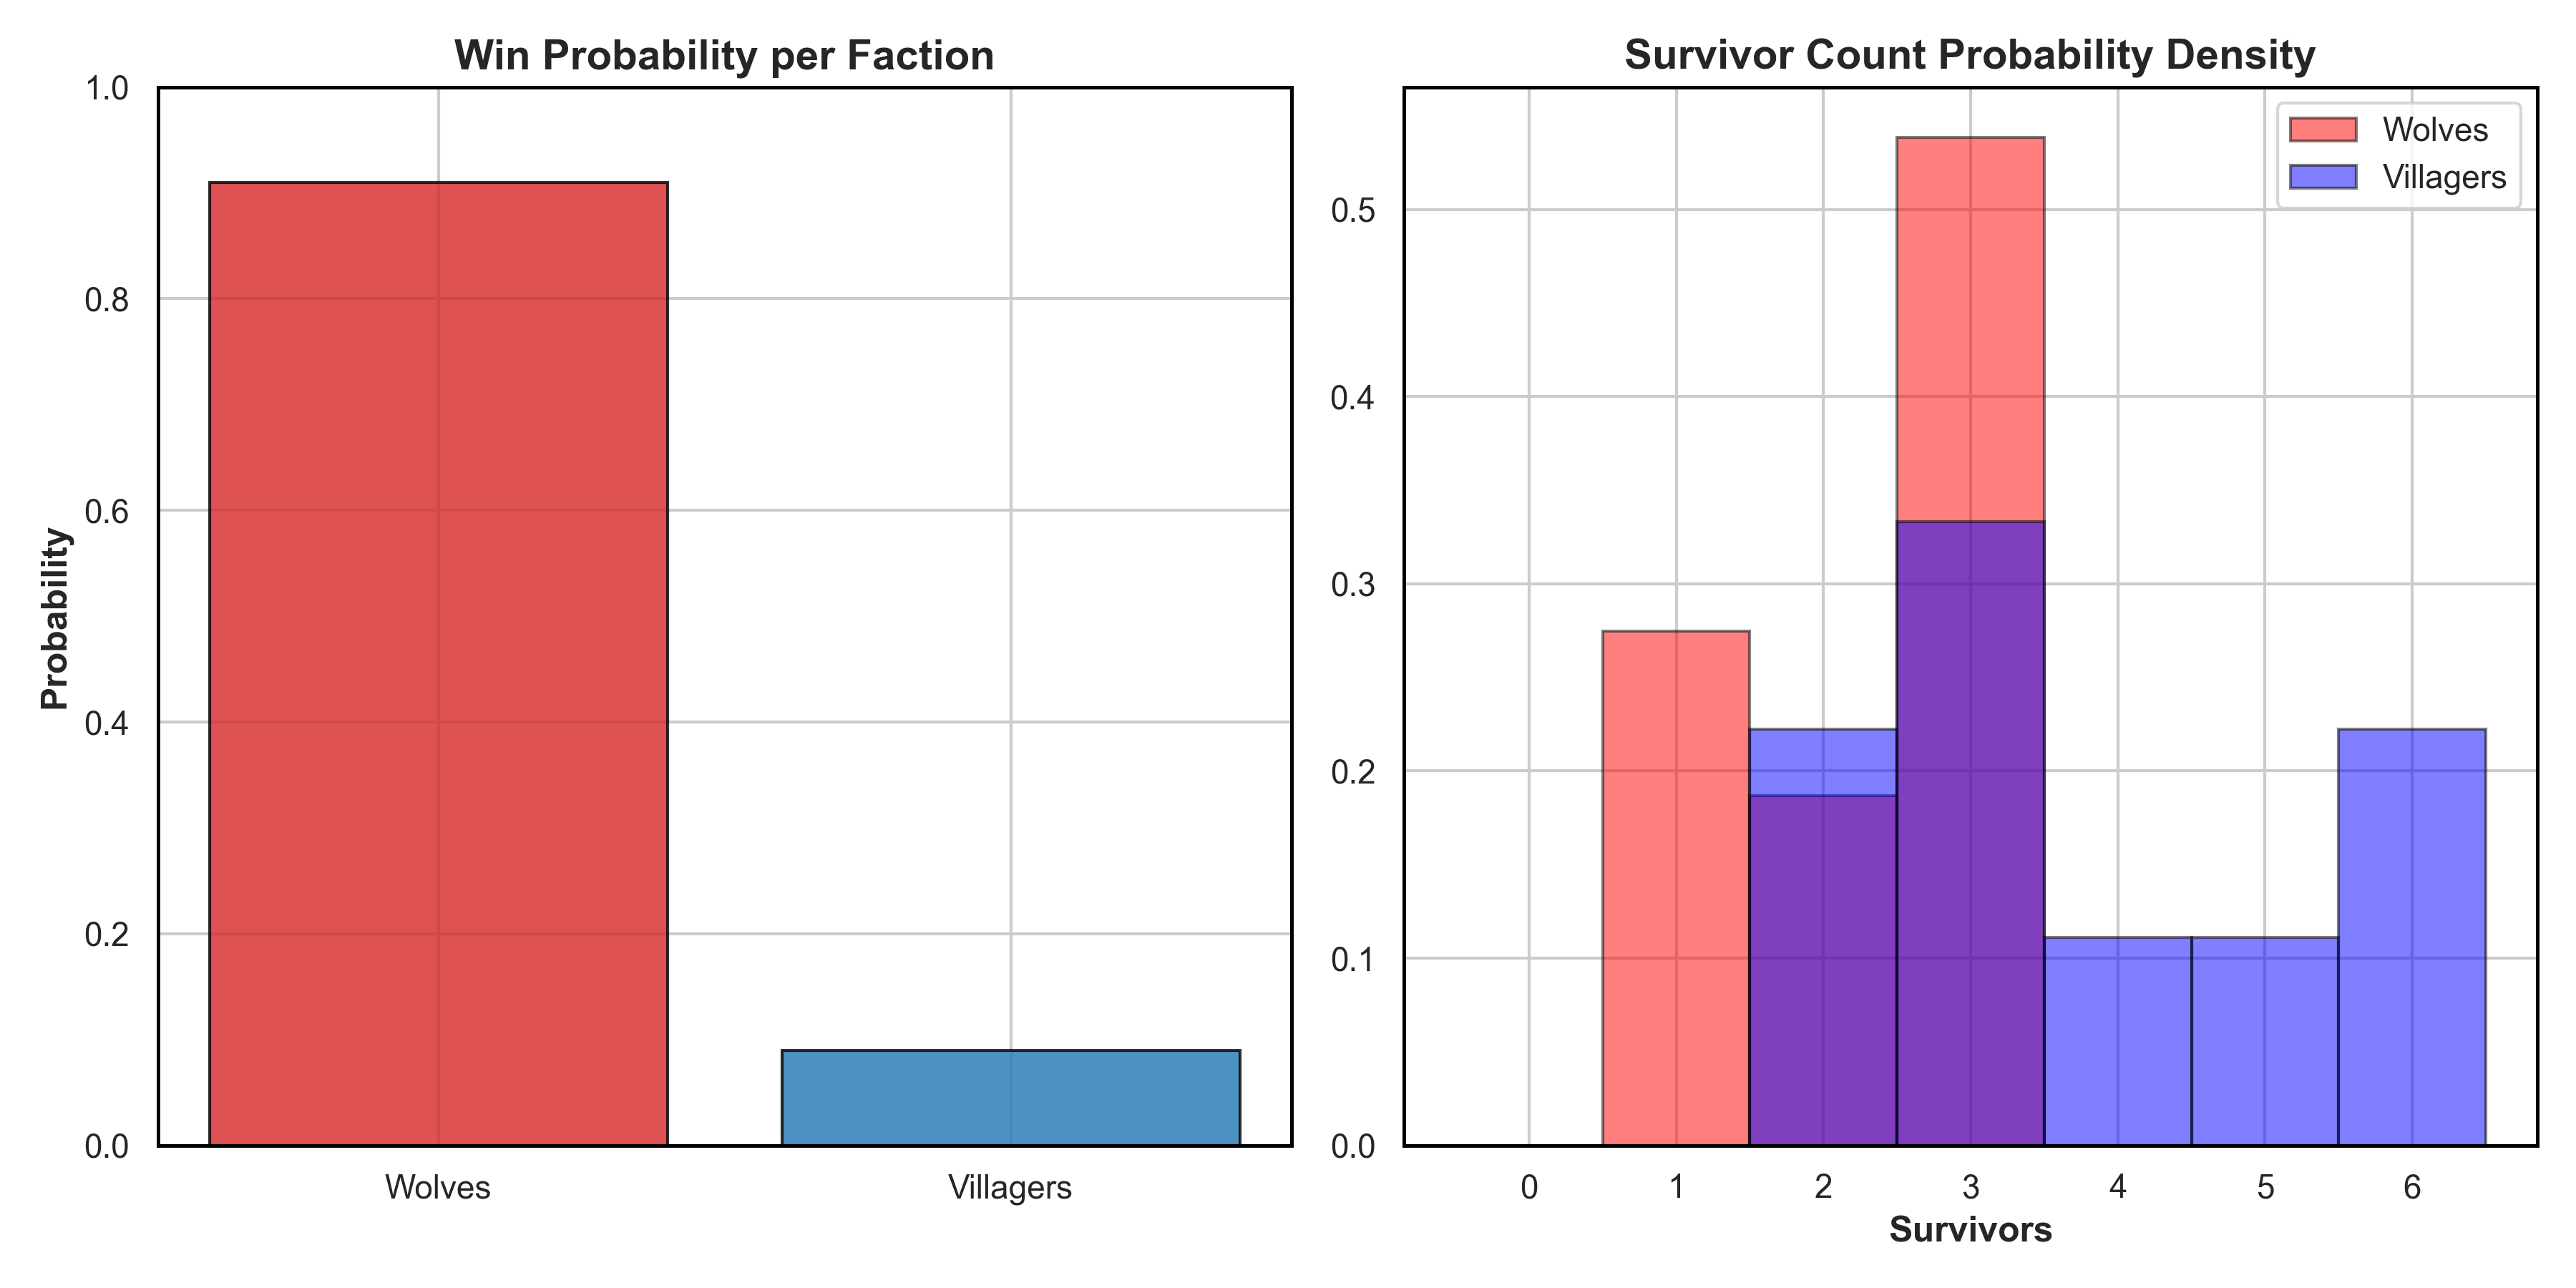
\includegraphics[width=1\textwidth]{images/game_results/symbolic_1.png}
    \caption{Win probability and survivor count density per faction.}
    \label{fig:symb_win_prob}
\end{figure}

Figure \ref{fig:symb_win_prob} demonstrates a severe structural imbalance in the pure symbolic setup. Despite a significant numerical disadvantage (3 vs. 12), the Wolf faction achieves a win rate exceeding 90\%. The survivor density further reflects this, showing that Wolves consistently maintain 1 to 3 survivors at the end of the game, whereas Villager victories are rare and yield higher survivor variance.

\begin{figure}[H]
    \centering
    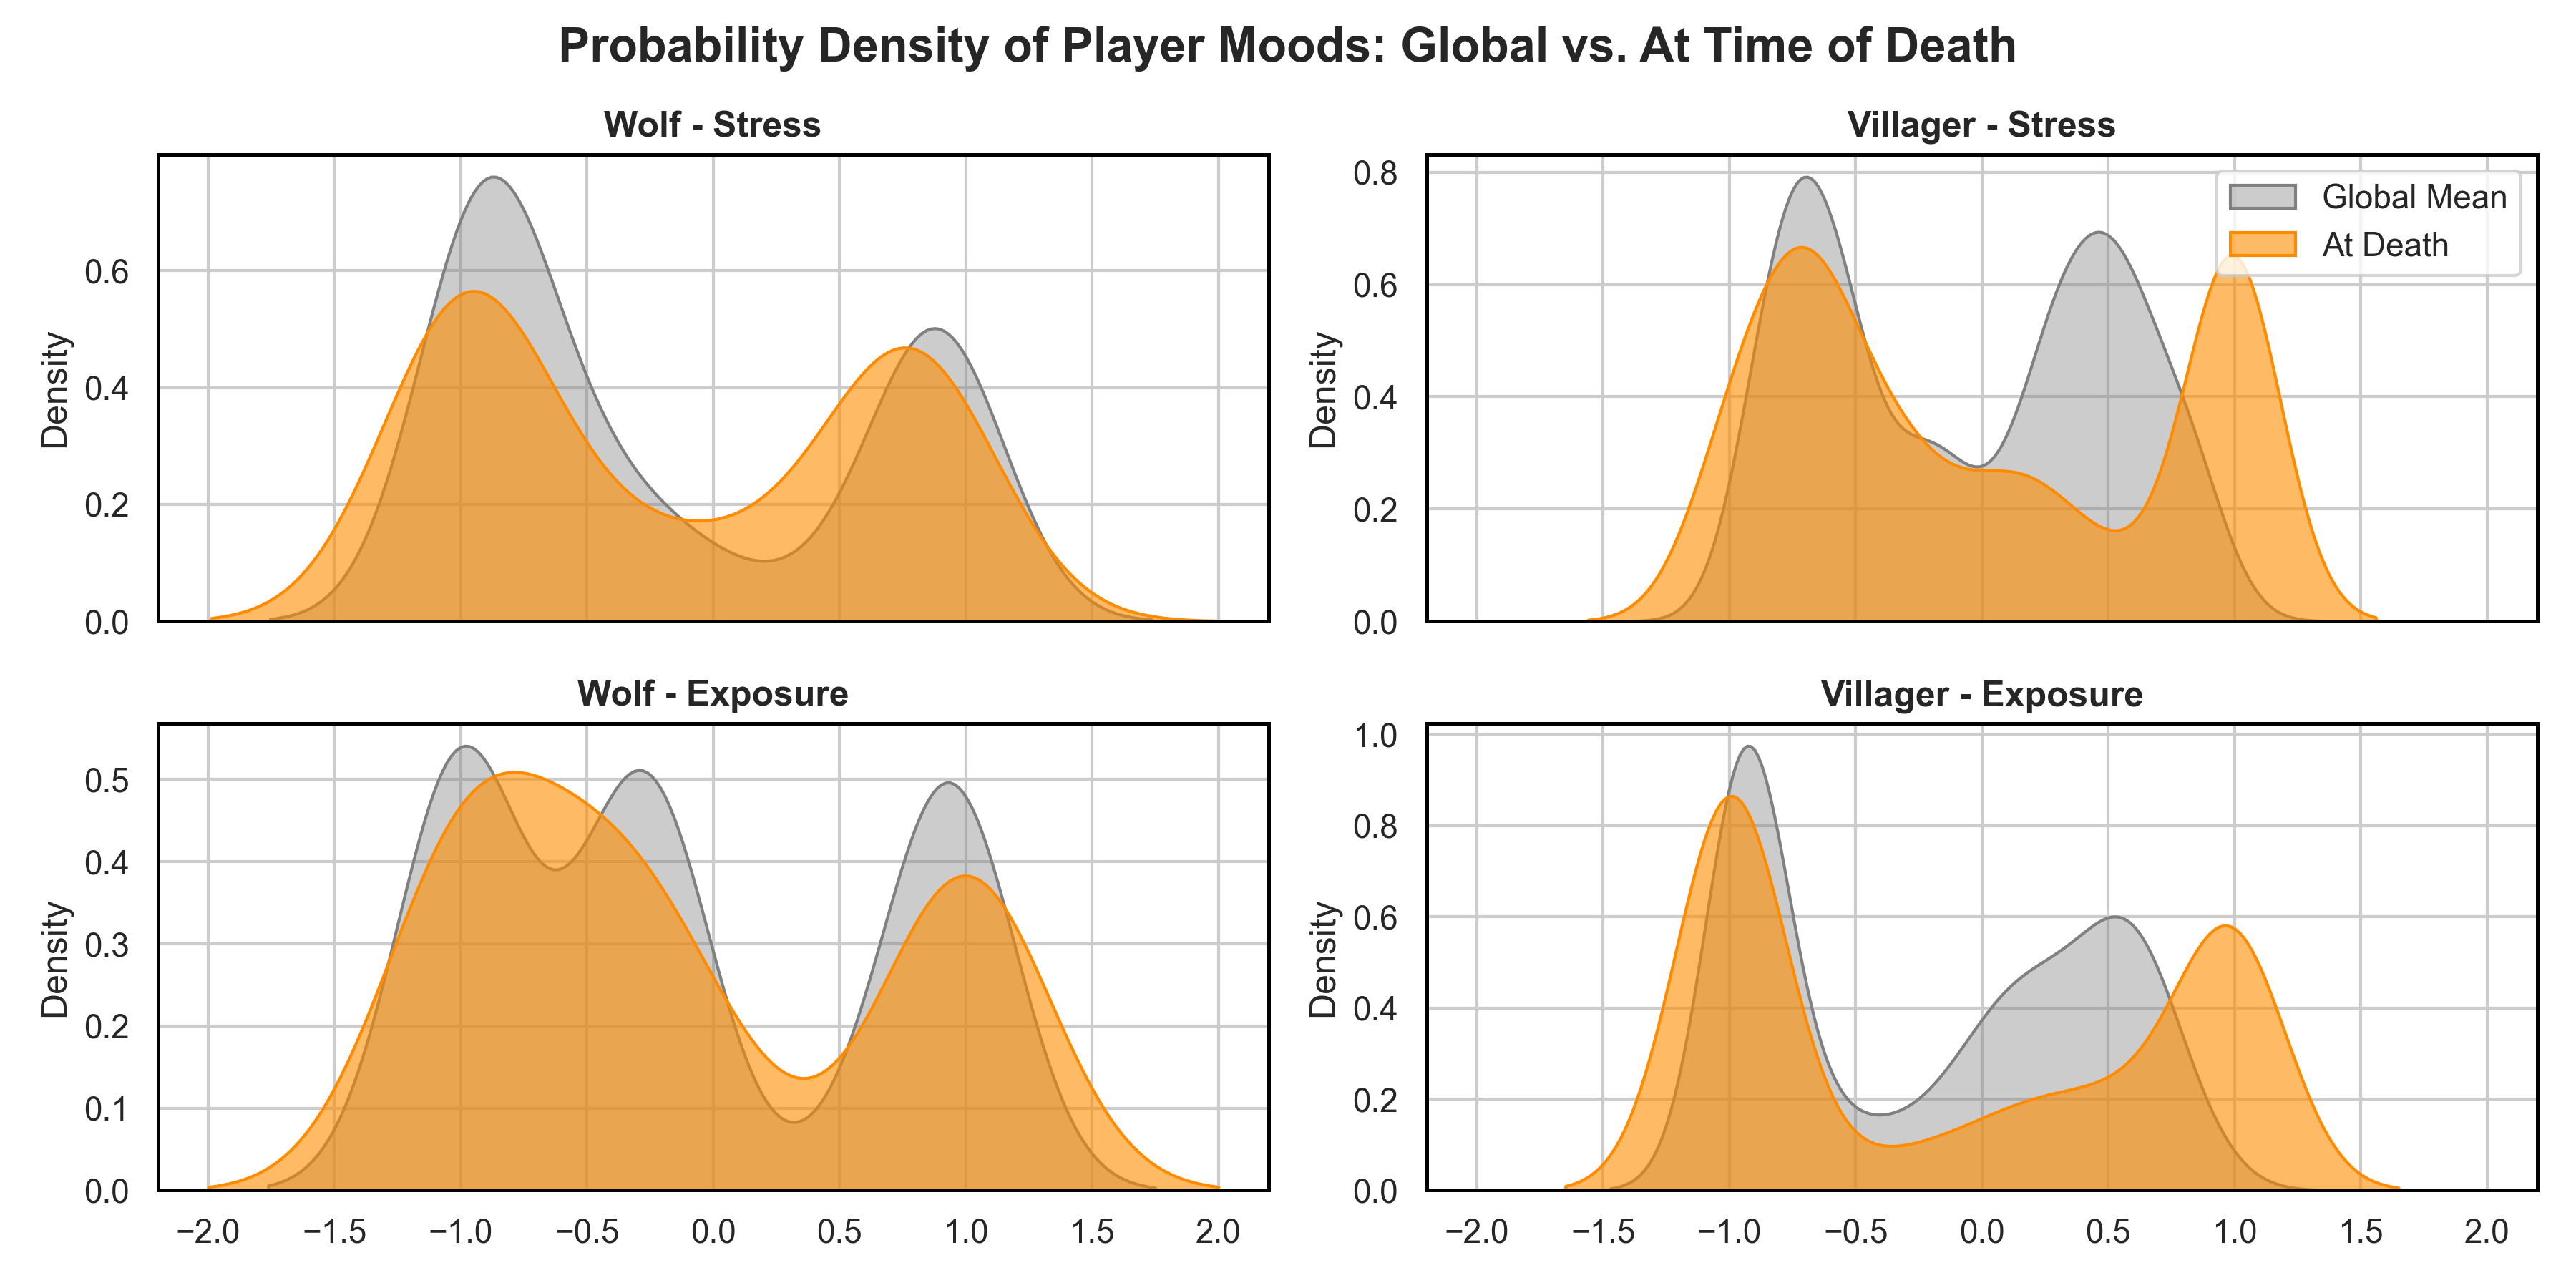
\includegraphics[width=1\textwidth]{images/game_results/symbolic_2.png}
    \caption{Density distributions of internal agent metrics (Stress and Exposure) comparing the global mean against the values recorded precisely at the time of the agent's death.}
    \label{fig:symb_metrics}
\end{figure}

Figure \ref{fig:symb_metrics} evaluates the internal state metrics of the agents. For both factions, but particularly for Villagers, the "At Death" density distribution (red) shows distinct right-side peaks compared to the "Global Mean" (blue). This indicates a strong positive correlation between elevated internal Stress/Exposure levels and in-game elimination, validating that the symbolic engine mathematically captures the danger state of the agents.

\begin{figure}[H]
    \centering
    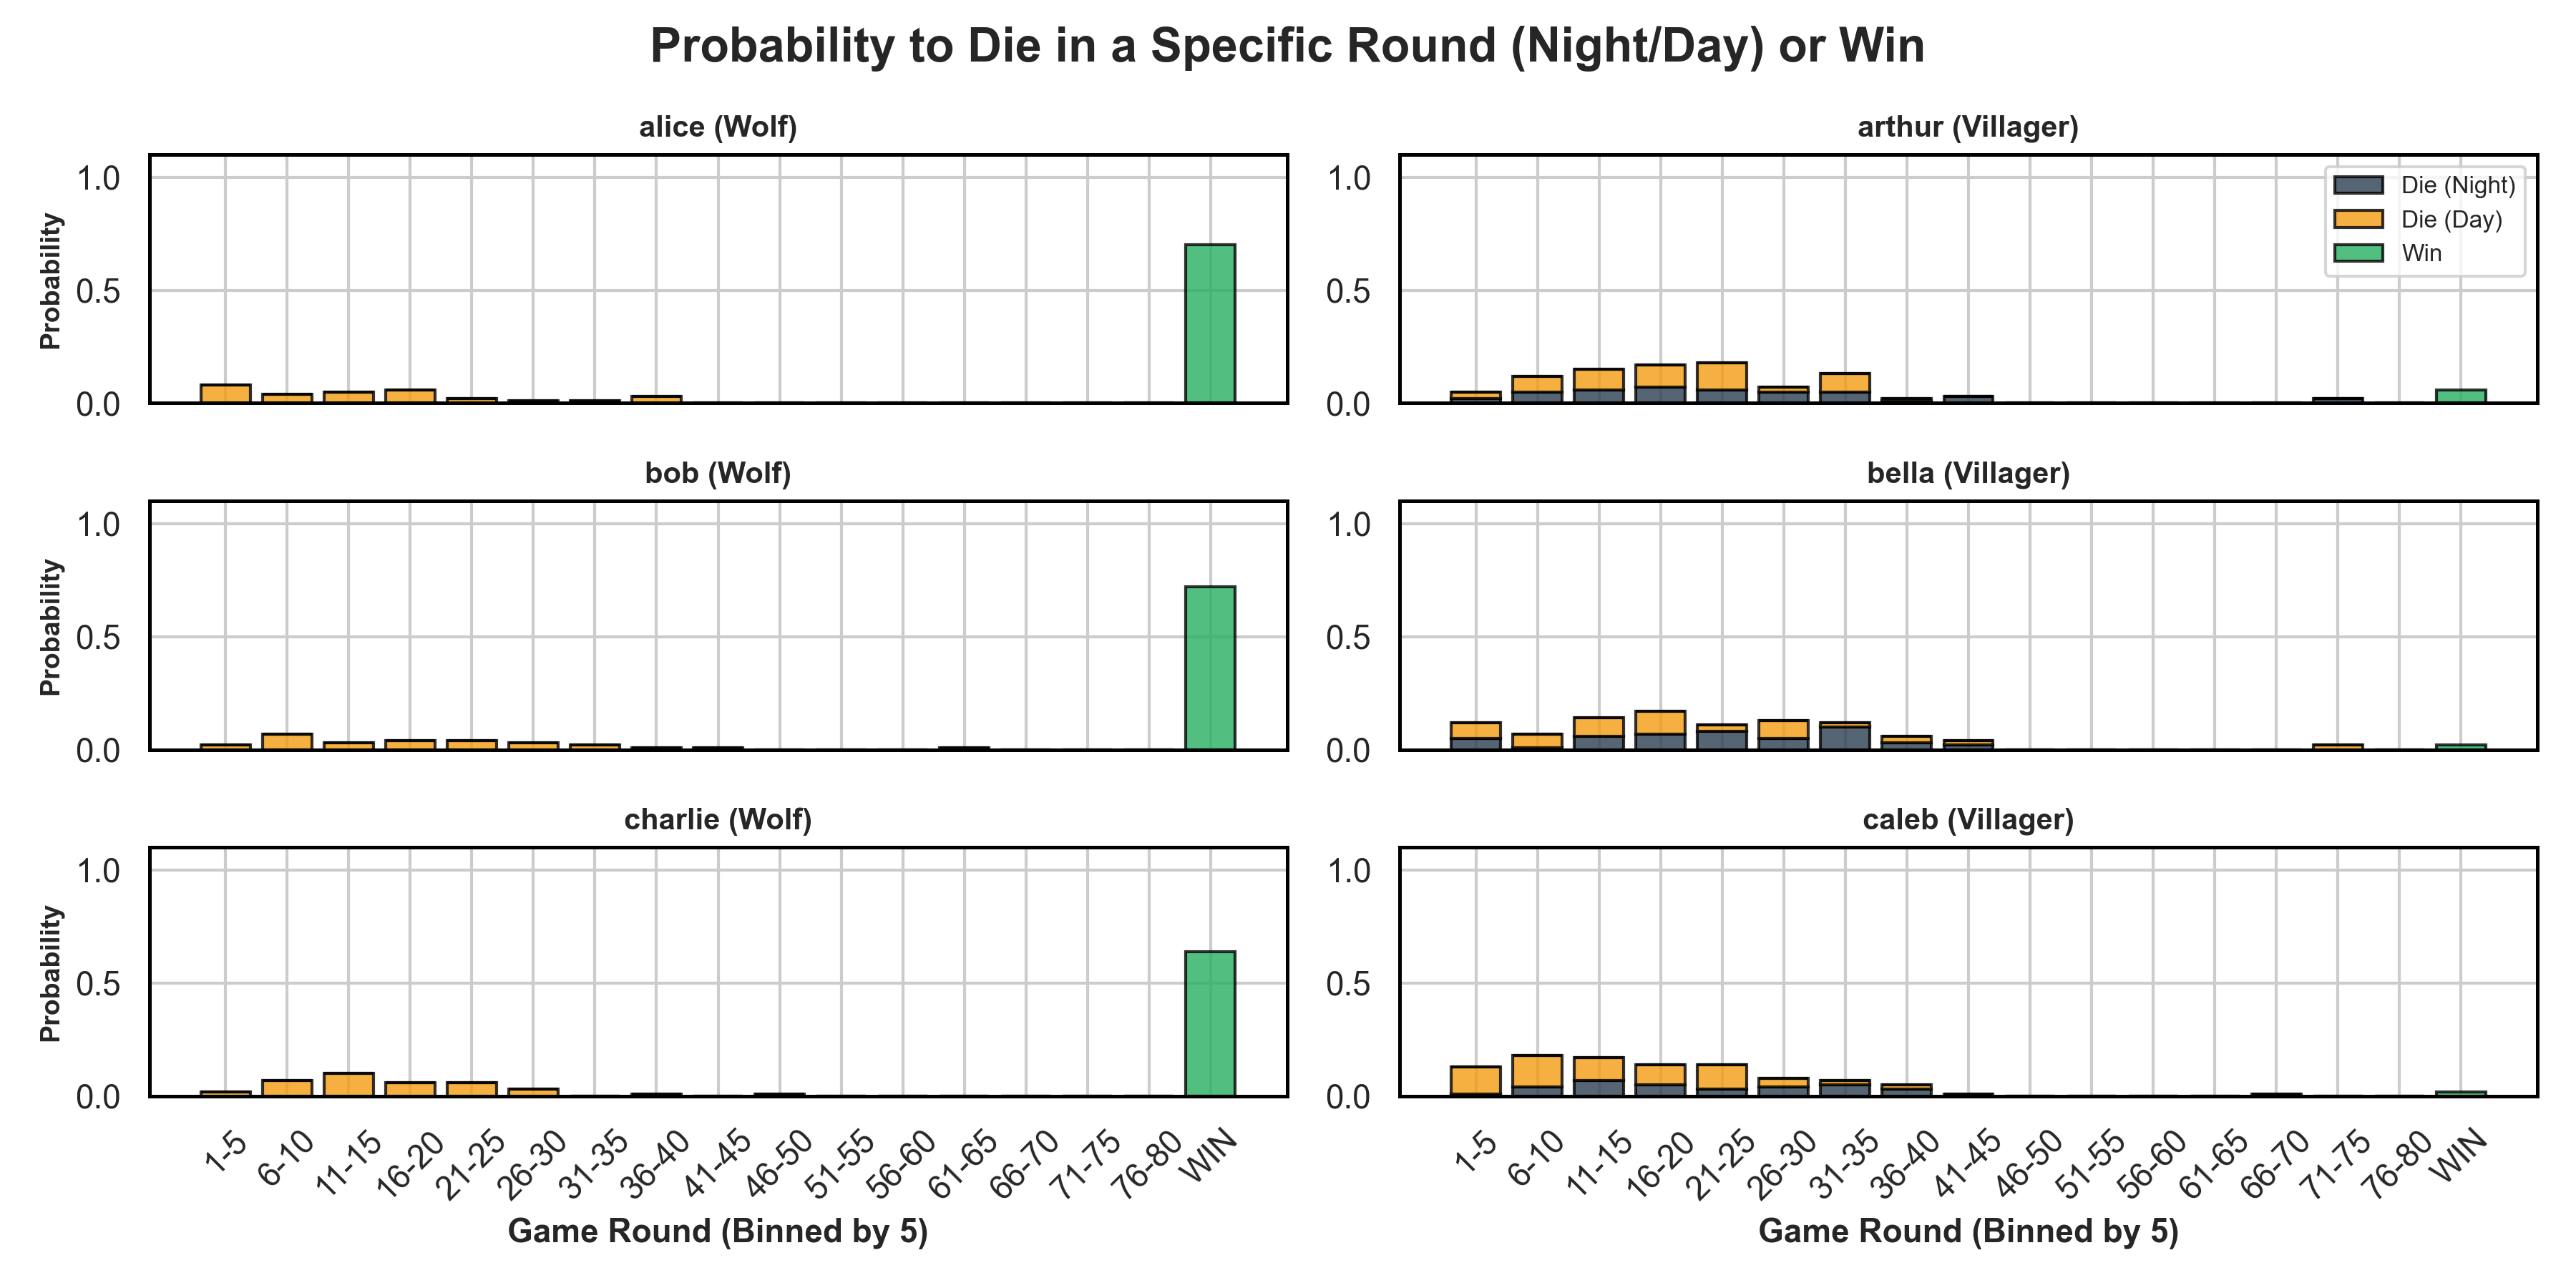
\includegraphics[width=1\textwidth]{images/game_results/symbolic_3.png}
    \caption{Probability distribution of player elimination across game rounds, segmented by Day/Night phases and ultimate Win state.}
    \label{fig:symb_survival}
\end{figure}

Finally, Figure \ref{fig:symb_survival} breaks down the temporal survival probabilities for specific agents. The data shows that Wolves (left column) experience minimal attrition, with very few deaths during the Day phase and zero at Night (confirming correct faction strategy implementation), overwhelmingly reaching the 'Win' state. Conversely, Villagers (right column) face steady, continuous elimination across the first 40 rounds, driven by a combination of Night (wolf attacks) and Day (incorrect lynching) phases.



\subsection{LLM-Driven Agents' Gameplay}


To test the LLM-driven agents (gemma4:31b), another set of simulations was conducted. Because processing natural language internal reasoning is computationally expensive, we scaled the game down to 12 players (3 Wolves and 9 Villagers). Even with this smaller roster, a single game took roughly 30 minutes using an externally hosted Ollama instance on an NVIDIA RTX 5090.

\begin{figure}[H]
    \centering
    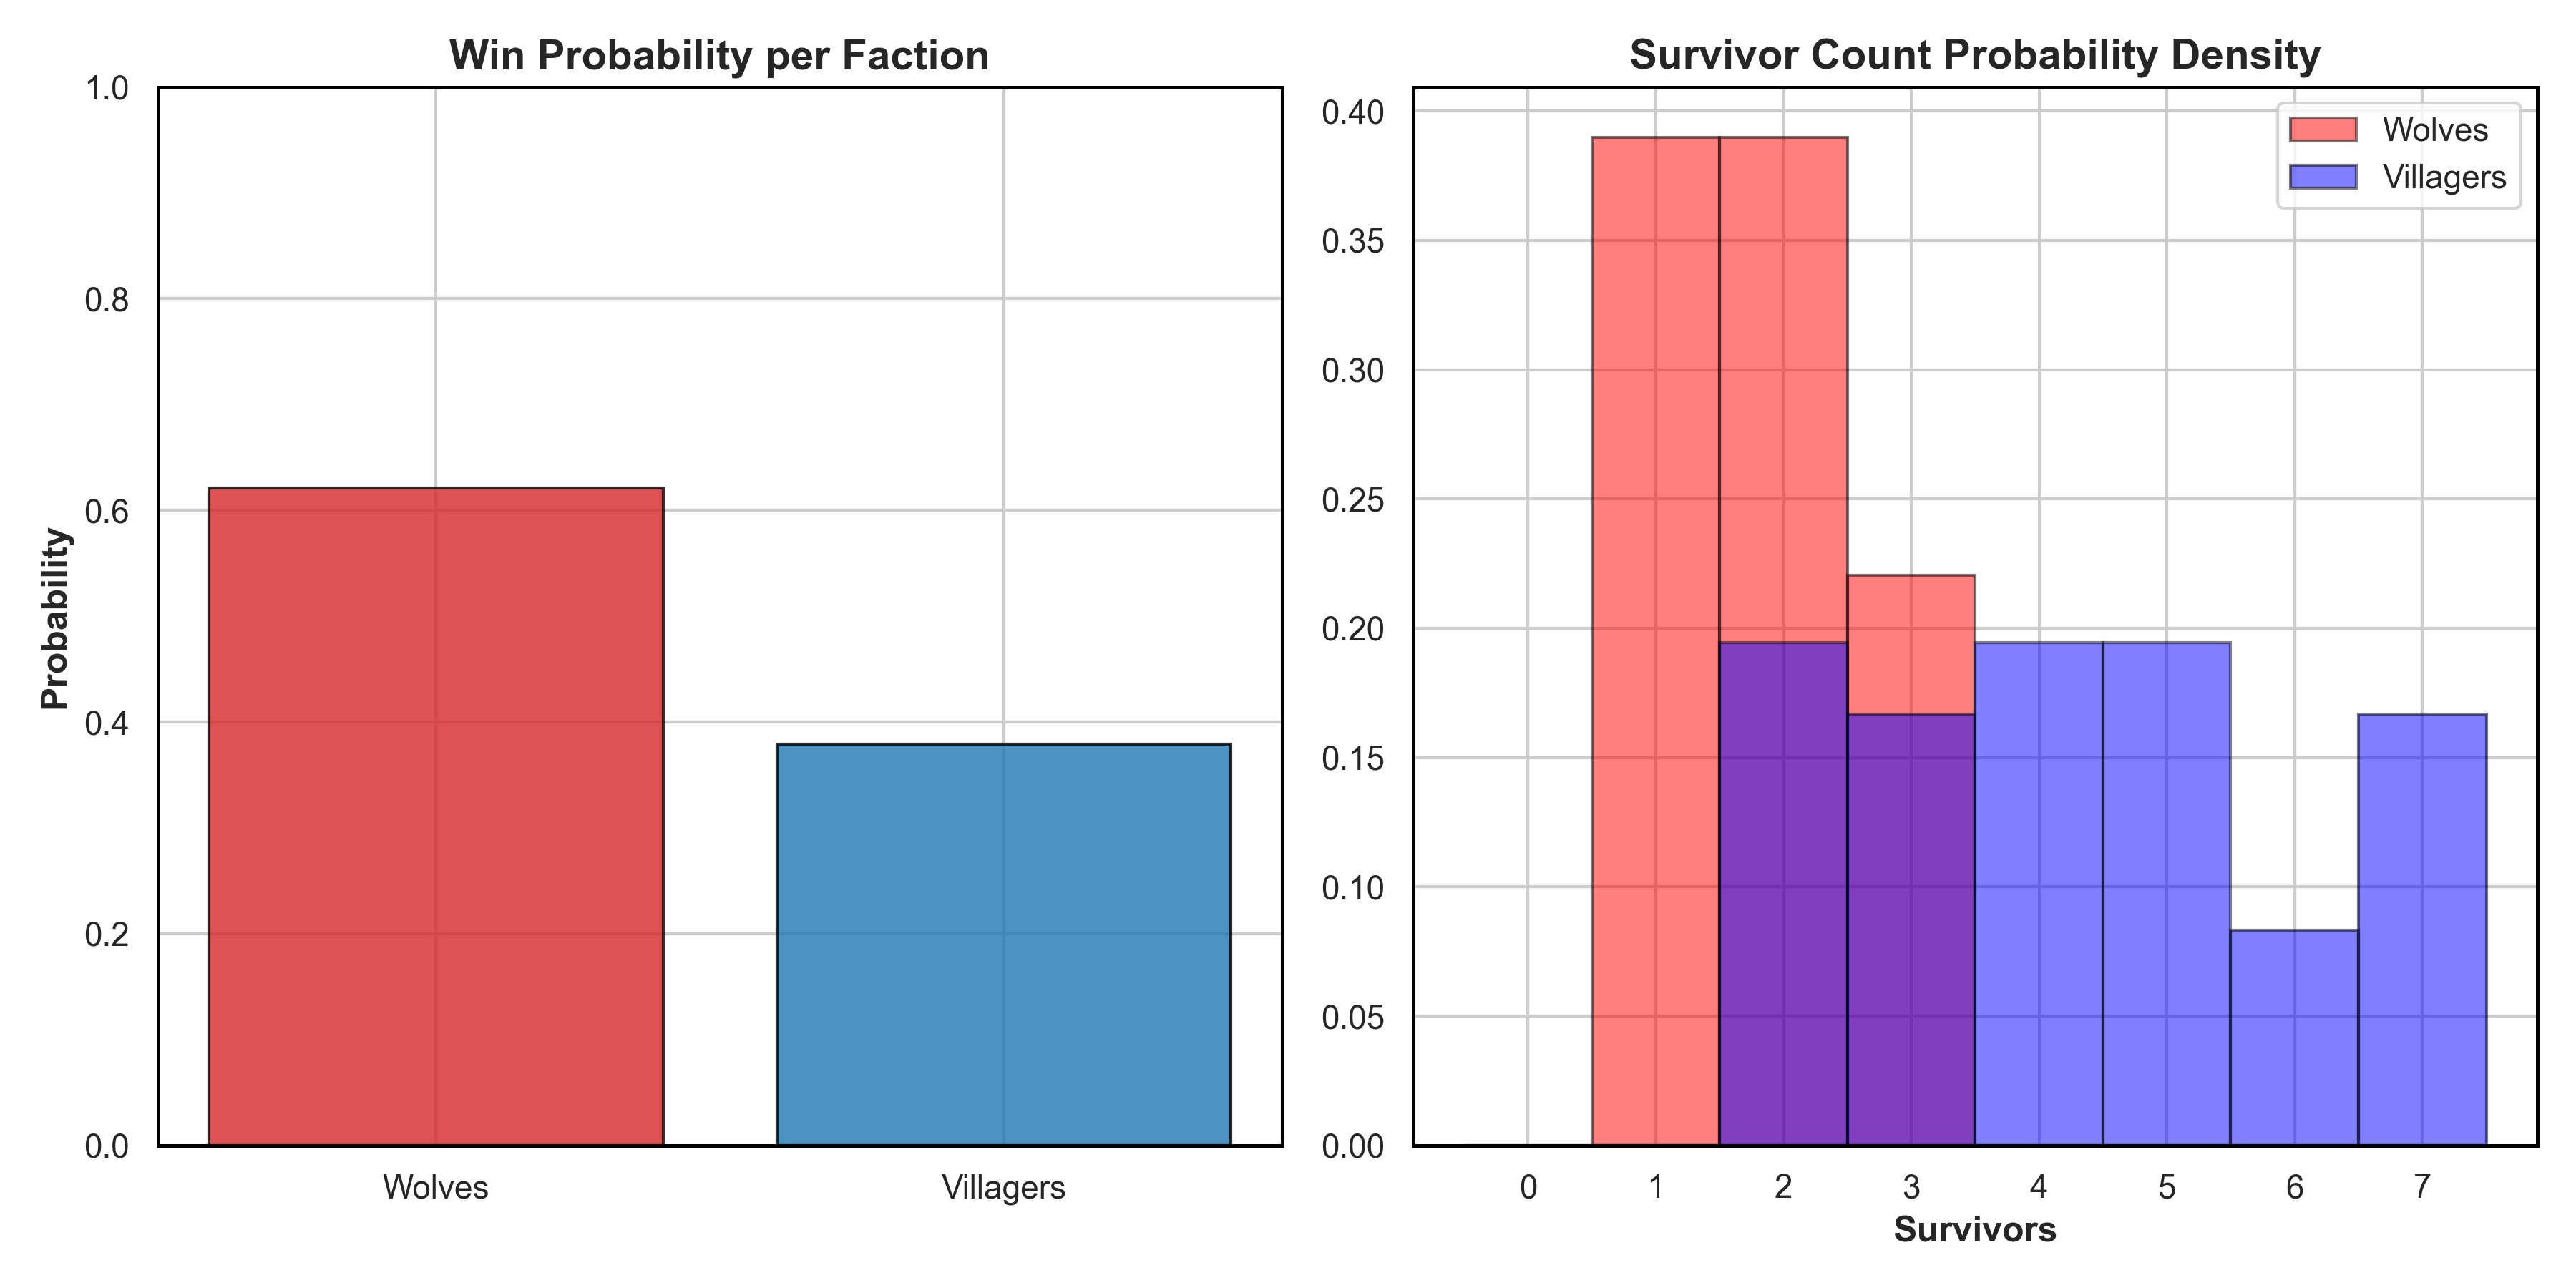
\includegraphics[width=1\textwidth]{images/game_results/llm_1.png}
    \caption{Win probability and survivor count density for LLM-driven agents.}
    \label{fig:llm_win_prob}
\end{figure}

Figure \ref{fig:llm_win_prob} shows that natural language reasoning drastically improves game balance. Compared to the purely symbolic baseline, the Wolf win rate drops from over 90\% to roughly 62\%, giving the Villagers a realistic 38\% chance to win.

\begin{figure}[H]
    \centering
    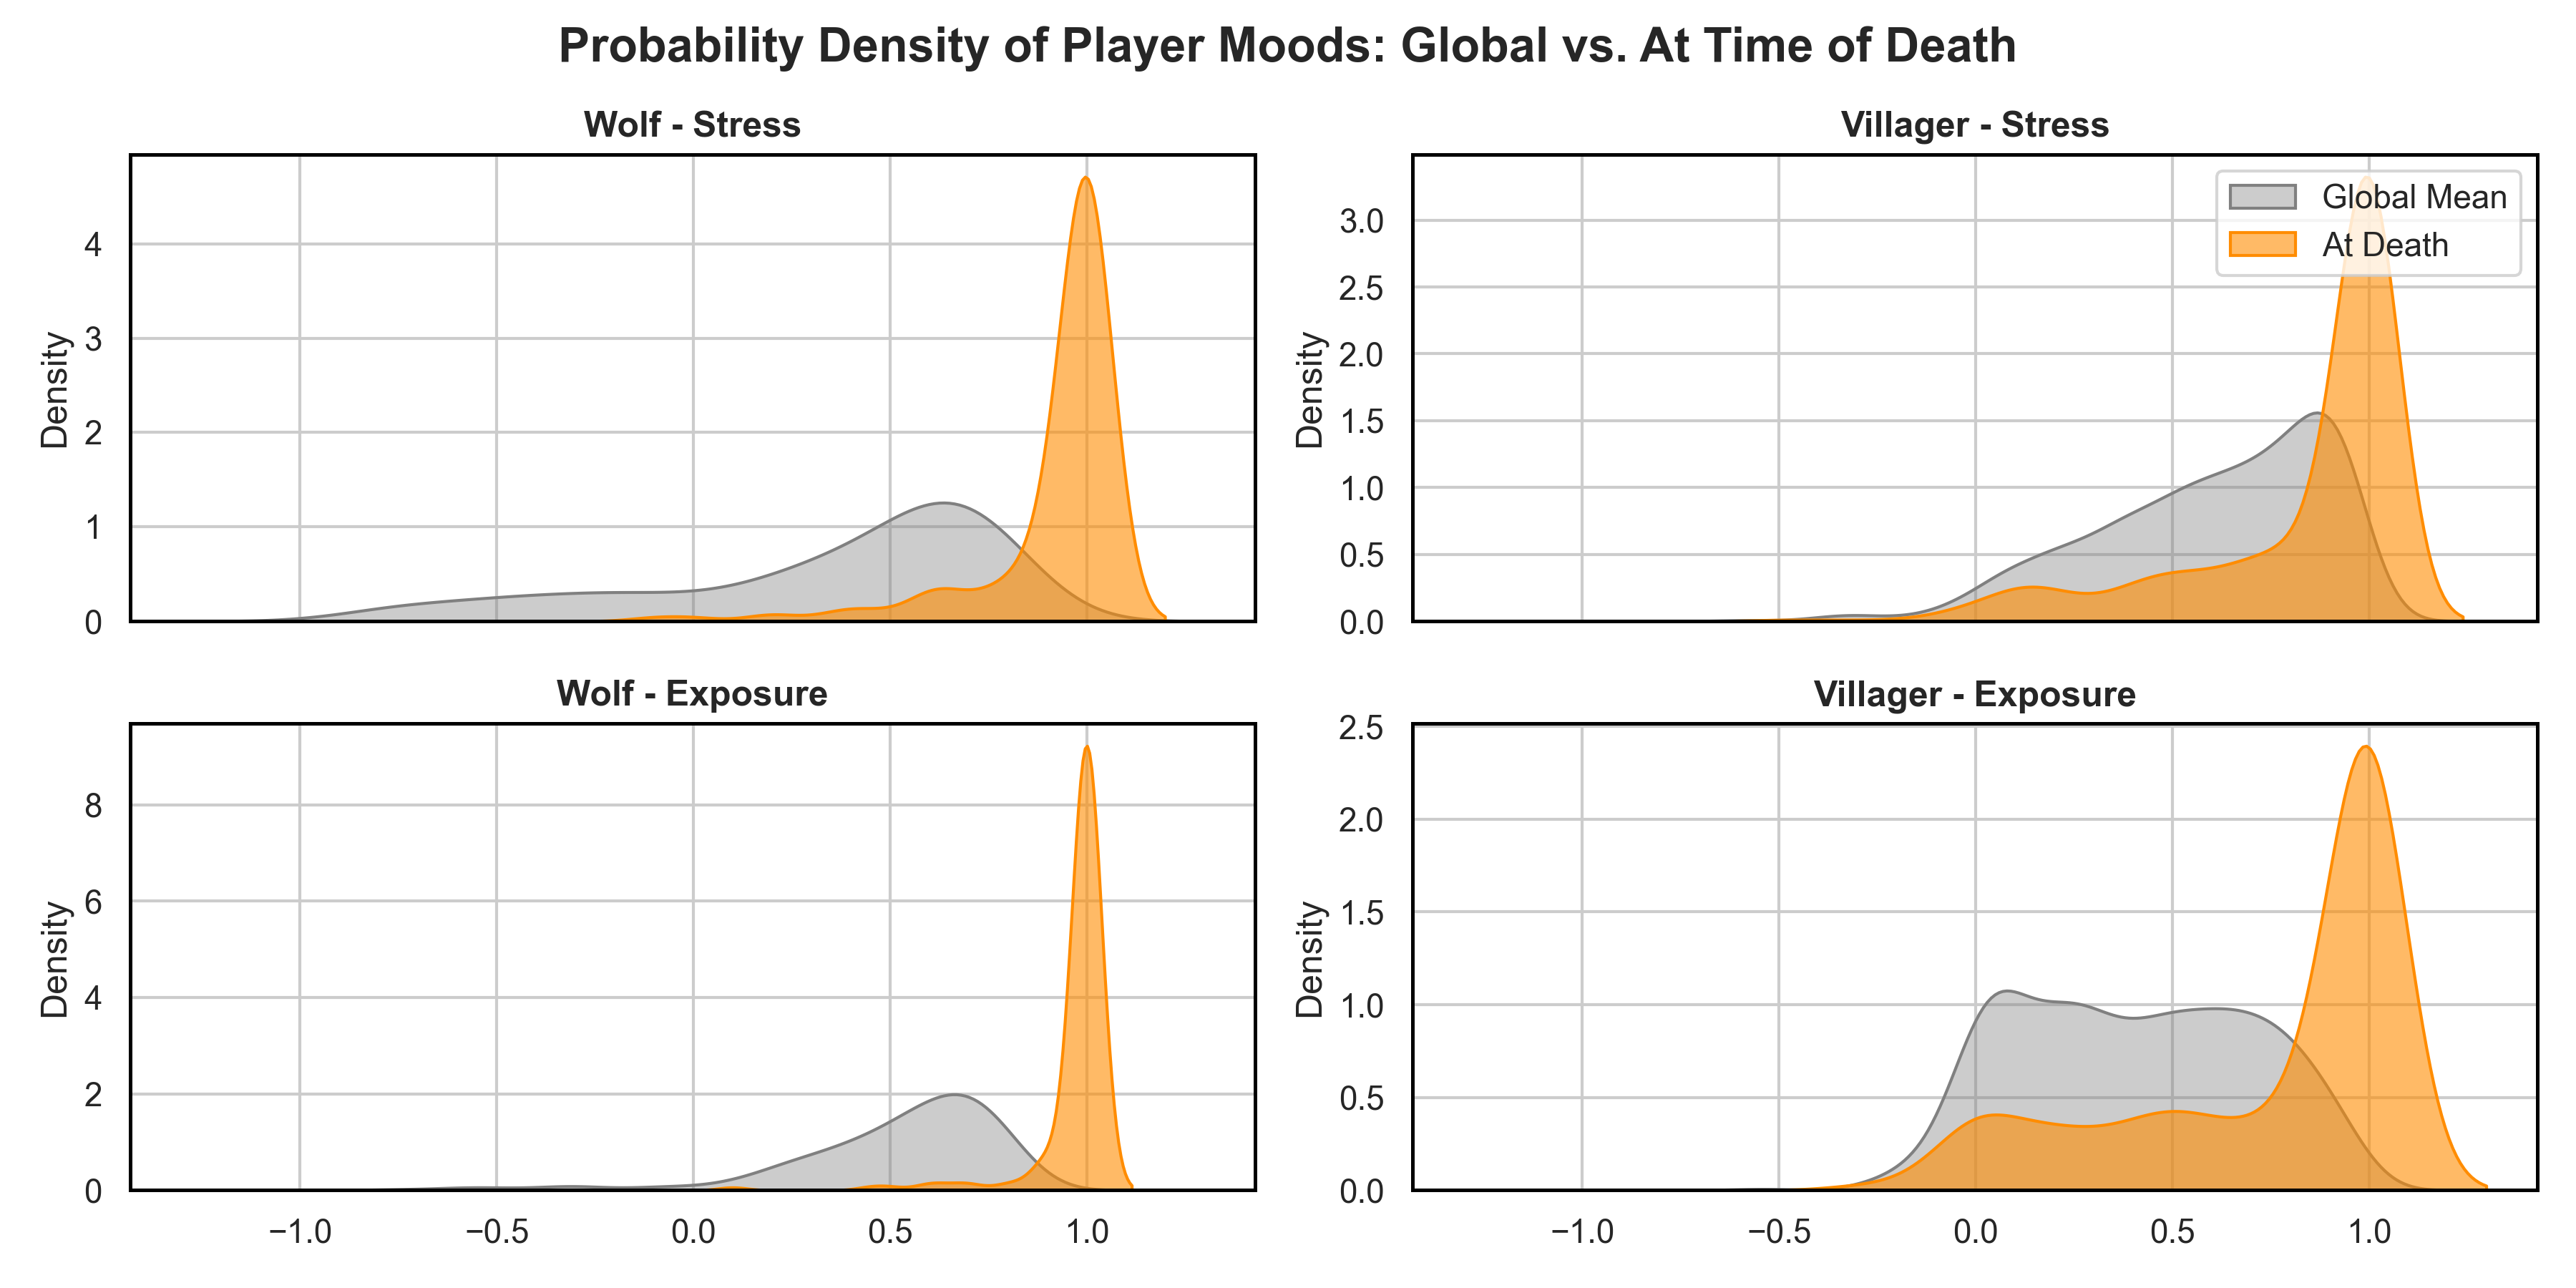
\includegraphics[width=1\textwidth]{images/game_results/llm_2.png}
    \caption{Density distributions of internal metrics (Stress and Exposure) for LLM-driven agents.}
    \label{fig:llm_metrics}
\end{figure}

Figure \ref{fig:llm_metrics} illustrates a major shift in how the agents handle internal metrics. Unlike the gradual curves of the symbolic engine, the LLM agents' stress and exposure spike sharply to 1.0 right before elimination. This proves the agents are highly aware of the game state: their metrics only max out when they correctly perceive they are in immediate, fatal danger.

\begin{figure}[H]
    \centering
    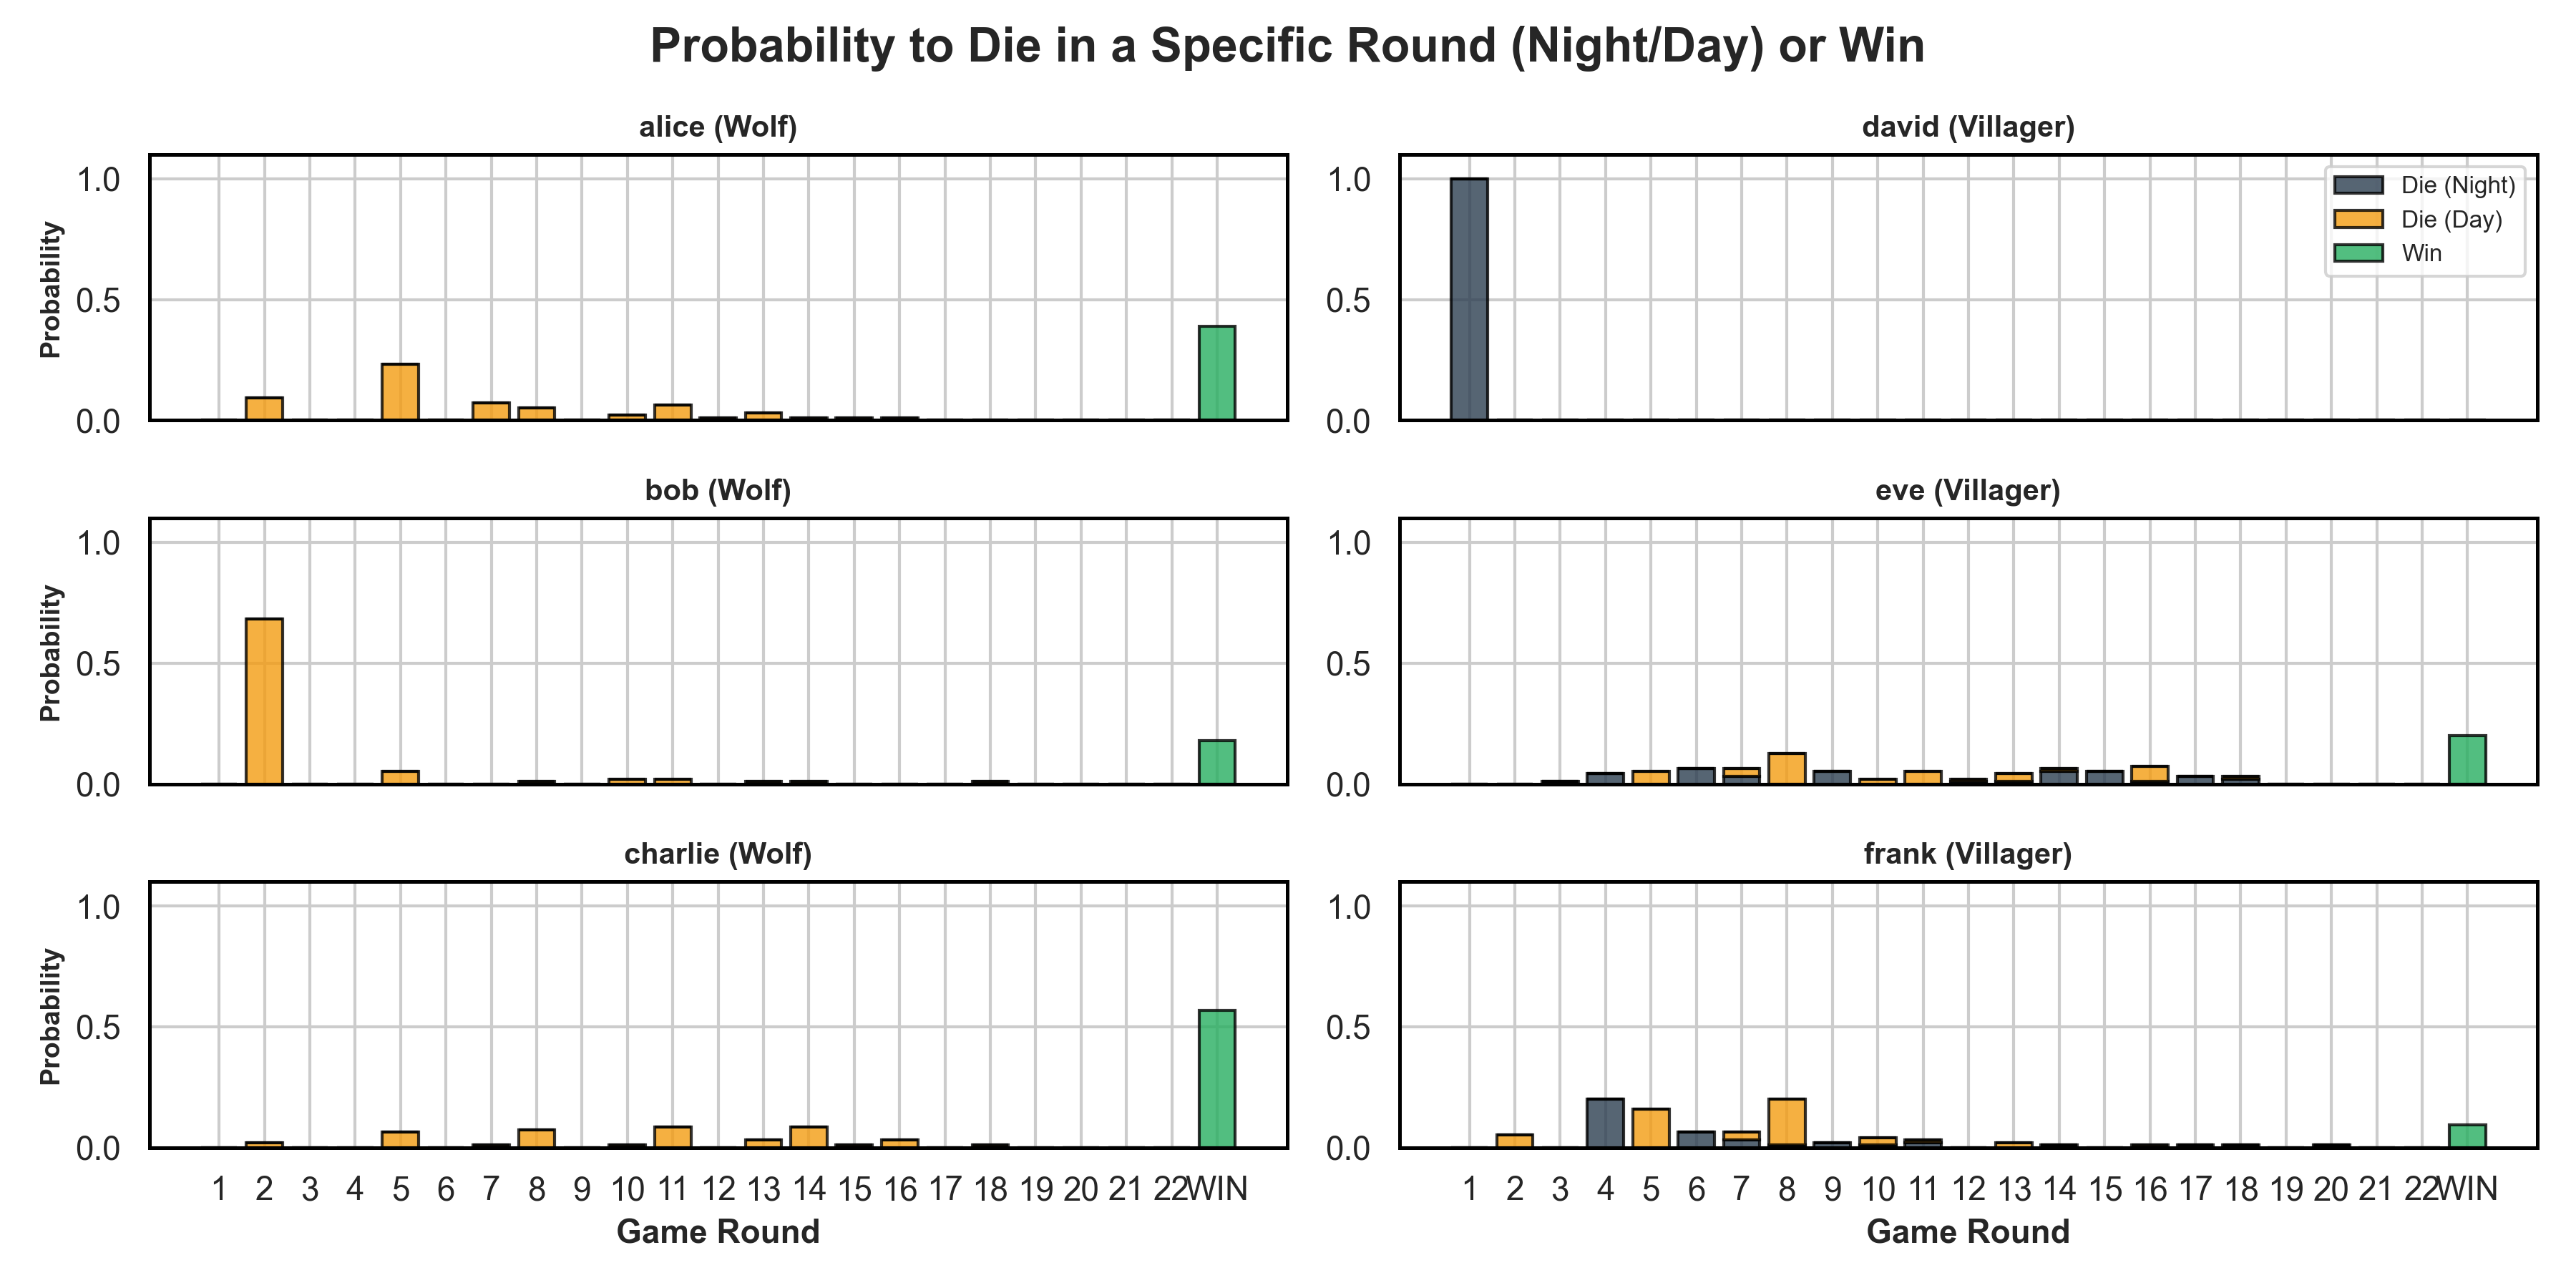
\includegraphics[width=1\textwidth]{images/game_results/llm_3.png}
    \caption{Probability distribution of player elimination across game rounds for LLM-driven agents.}
    \label{fig:llm_survival}
\end{figure}

Finally, Figure \ref{fig:llm_survival} highlights two distinct LLM behaviors. First, the games resolve much faster, typically ending within 20 rounds instead of 80. Second, the model shows severe targeting biases: the Villager 'david' is killed on Night 1 in almost every game, while the Wolf 'bob' is frequently lynched on Day 2. This suggests the underlying LLM relies on inherent lexical or contextual biases when selecting targets.

\paragraph{Emergent Biases in LLM Targeting}

The targeting behaviors observed in Figure \ref{fig:llm_survival} reveal a critical vulnerability in LLM-driven simulation: the manifestation of severe lexical biases. Despite strictly randomizing the order of player names in the prompt context and ensuring all agents started Round 1 with identical, "empty" internal states, the LLMs exhibited near-deterministic targeting. 

Specifically, the Villager 'david' was universally targeted by the Wolves on Night 1. Since the Wolf faction acts first and lacks any prior game context, this suggests the model defaulted to targeting the first alphabetically available Villager in its generated list.

More interestingly, the Wolf 'bob' was overwhelmingly targeted for lynching on Day 1. A hypothesized reason for this bypasses alphabetical sorting (which would target 'alice') and instead points to artifacts within the LLM's pre-training dataset. 

In computer science and cryptography literature, stereotypical transactional examples almost universally follow the format "Alice performs an action on Bob." Given that the system prompt explicitly commands the model to execute a target (\textit{"TASK: Cast your vote... Choose the player you want to eliminate"}), the LLM may inherently associate 'Bob' with the semantic role of the passive target or victim. These emergent behaviors demonstrate that without strict alignment safeguards, generative agents will substitute rational gameplay strategy with linguistic heuristics learned during pre-training.